\section{Full contrast tables}
\label{app:tables}

All tables in this appendix are persona-paired ($n{=}96$), report $K{=}0$ minus $K{=}5$ unless
a pair is named explicitly, and never average the two graders. GRPO \Kf{} is right-censored at
iteration~5. The complete per-iteration, per-instrument tables (with bootstrap CIs and raw
Wilcoxon $p$) are the \texttt{tables/*.md} files of the paper's fixture (rendered by the tracked
EDA under \texttt{eda/results/<family>/tables/}); the rows here are the ones the text uses.

\begin{figure*}[t]
  \centering
  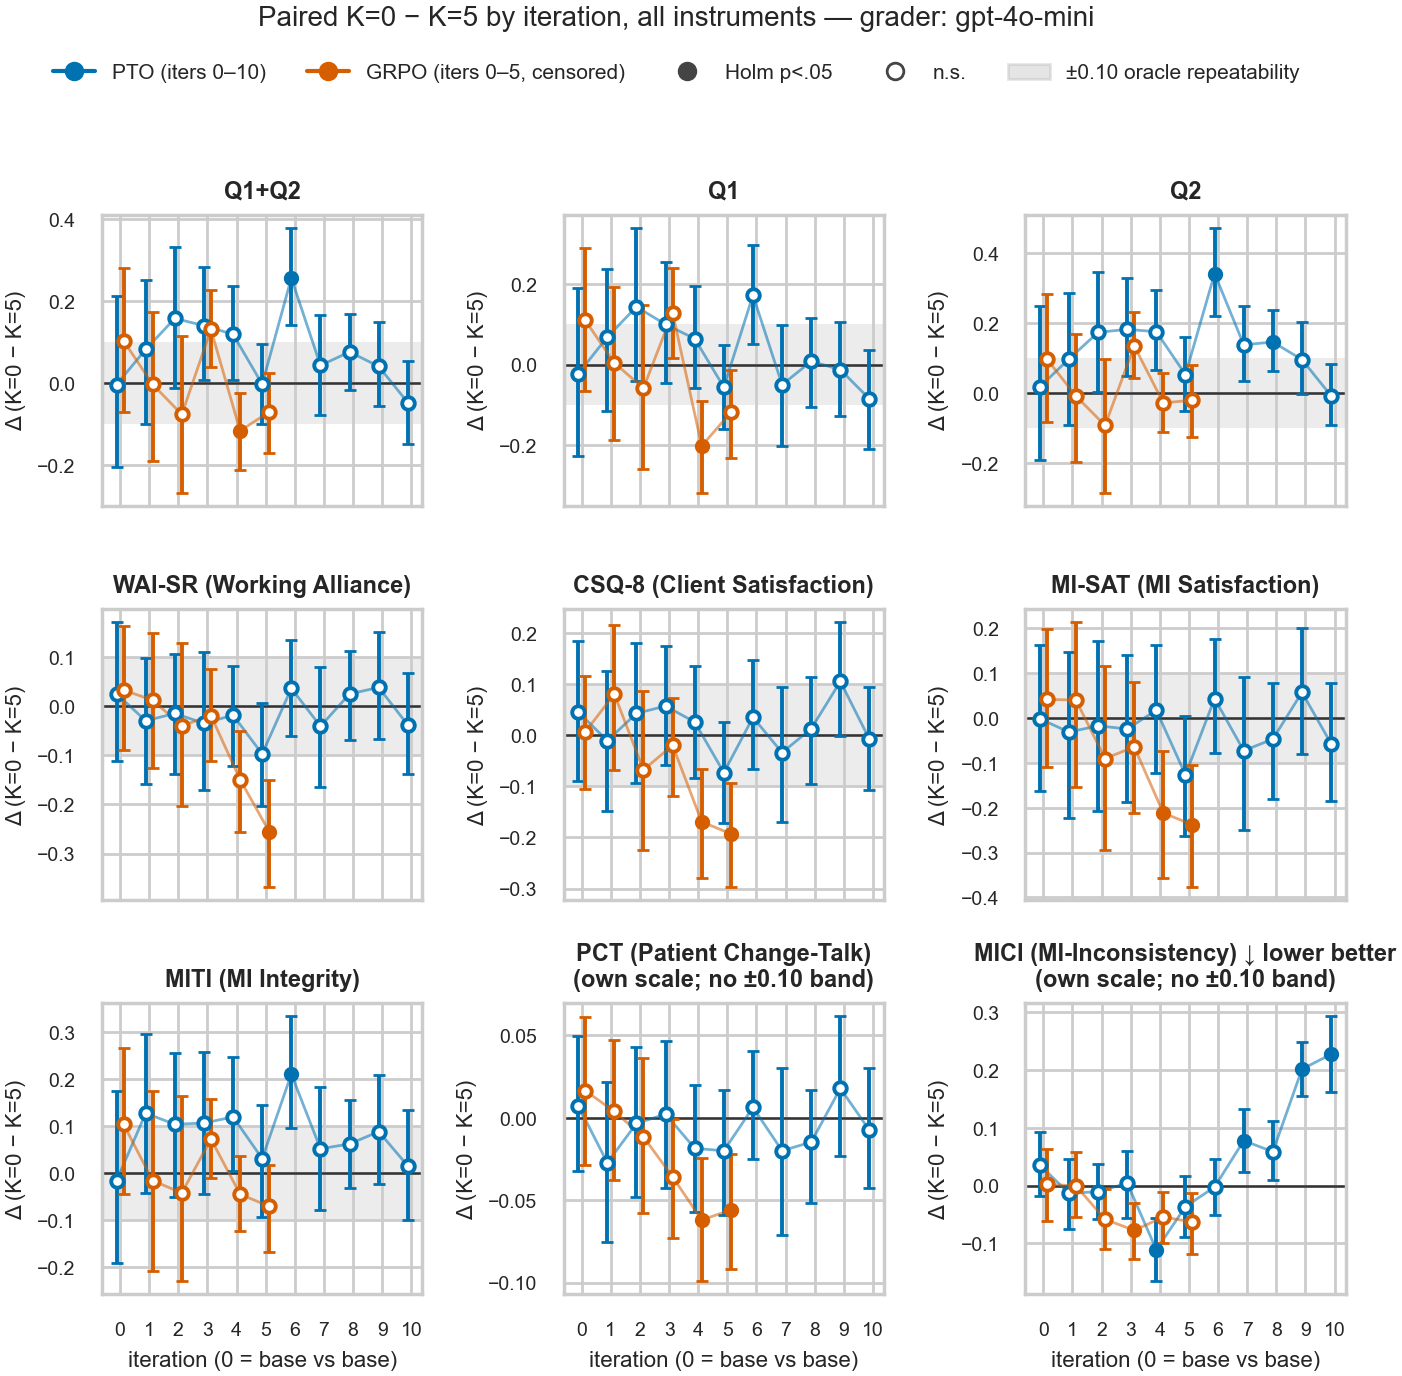
\includegraphics[width=\textwidth]{figures/k_contrast_headline_fig_grid_primary.png}
  \caption{Persona-paired $K{=}0$ minus $K{=}5$ by iteration for all nine instruments under the
    training oracle (\primaryjudge{}); PTO to iteration~10, GRPO to~5. Filled markers clear Holm
    correction across iterations; the $\pm 0.10$ band is drawn for the Likert rubrics only. MICI
    is lower-better, so a positive contrast means \Kz{} is more MI-inconsistent.}
  \label{fig:grid:primary}
\end{figure*}

\begin{figure*}[t]
  \centering
  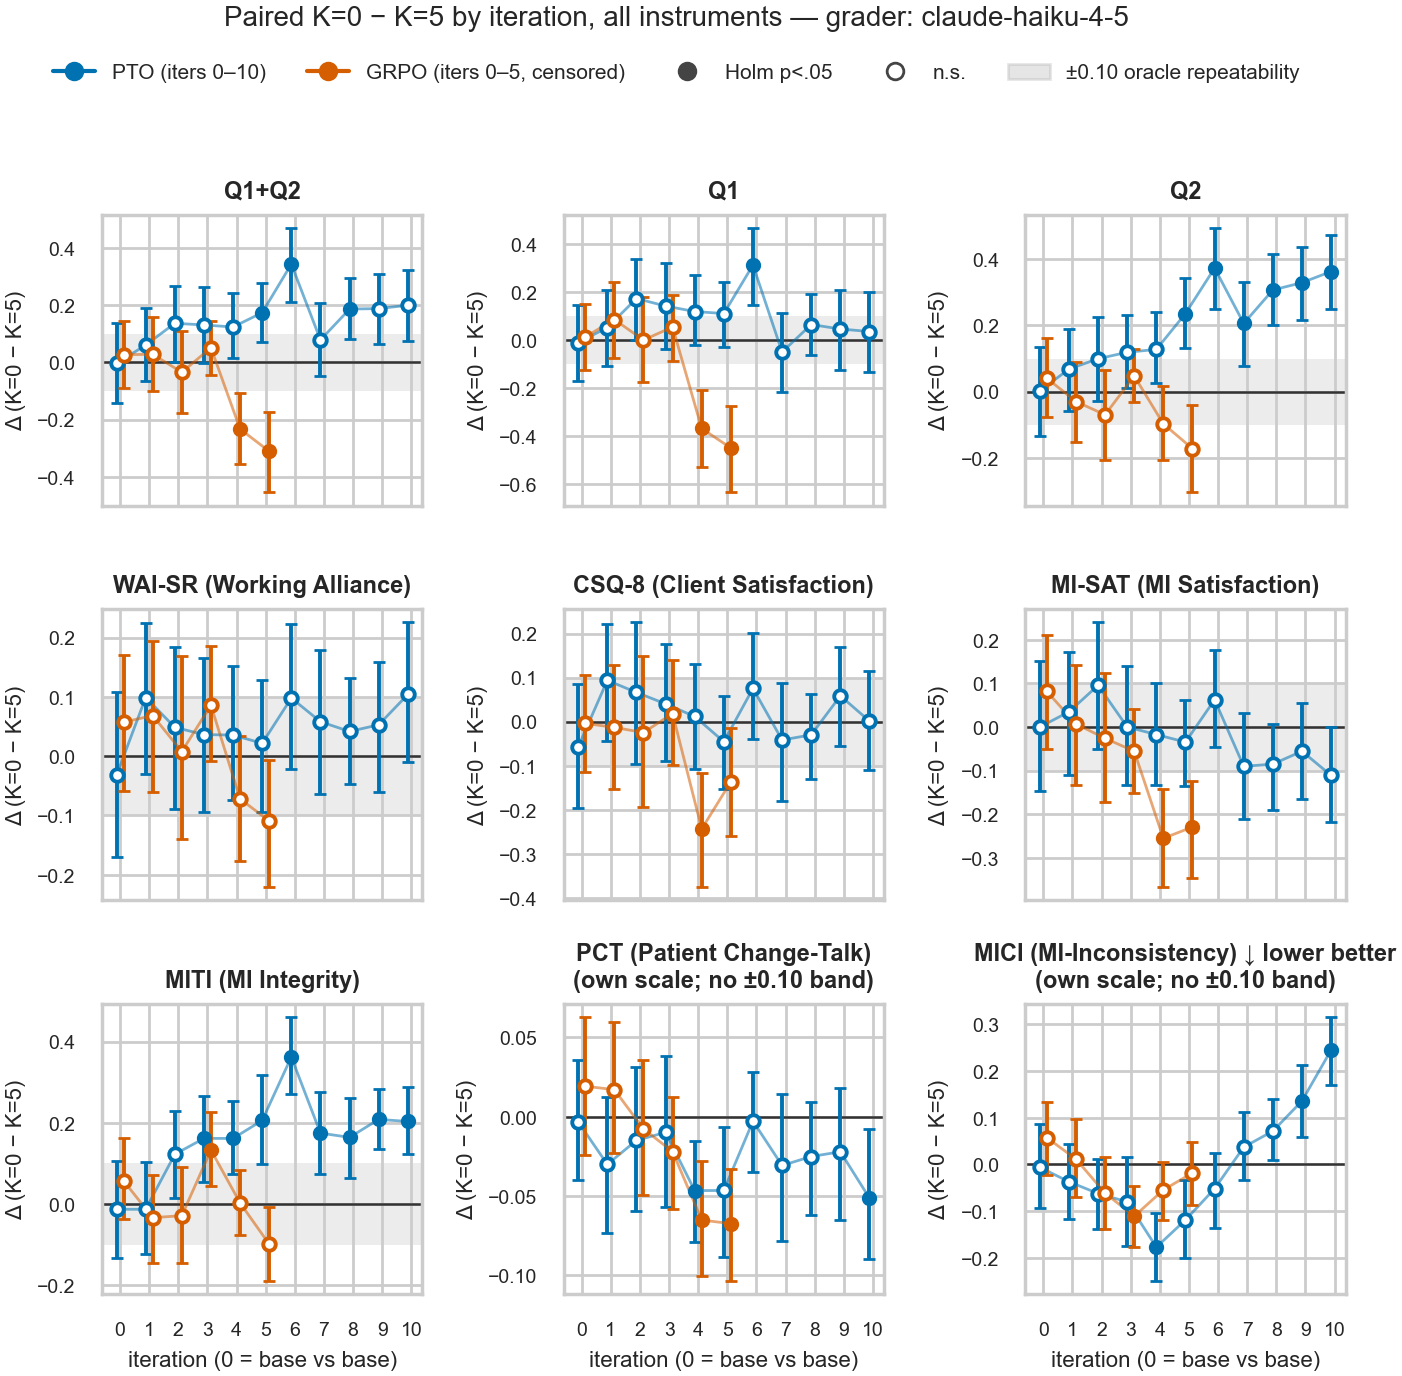
\includegraphics[width=\textwidth]{figures/k_contrast_headline_fig_grid_heldout.png}
  \caption{As Figure~\ref{fig:grid:primary}, under the held-out judge (\heldoutjudge{}).}
  \label{fig:grid:heldout}
\end{figure*}

\begin{table*}[t]
  \centering\footnotesize
  \setlength{\tabcolsep}{3pt}
  \begin{tabular}{@{}l ccr ccr ccr ccr@{}}
    \toprule
    & \multicolumn{3}{c}{PTO, oracle (10 iters)} & \multicolumn{3}{c}{PTO, held-out (10)} & \multicolumn{3}{c}{GRPO, oracle (5)} & \multicolumn{3}{c}{GRPO, held-out (5)} \\
    \cmidrule(lr){2-4}\cmidrule(lr){5-7}\cmidrule(lr){8-10}\cmidrule(lr){11-13}
    instrument & sig. & at iterations & $\bar\Delta$ & sig. & at iterations & $\bar\Delta$ & sig. & at iterations & $\bar\Delta$ & sig. & at iterations & $\bar\Delta$ \\
    \midrule
Q1Q2 & 1/0 & \scriptsize K0: 6 & $+0.087$ & 3/0 & \scriptsize K0: 5 6 8 & $+0.162$ & 0/1 & \scriptsize K5: 4 & $-0.026$ & 0/2 & \scriptsize K5: 4 5 & $-0.100$ \\
Q1 & 0/0 &  & $+0.035$ & 1/0 & \scriptsize K0: 6 & $+0.100$ & 0/1 & \scriptsize K5: 4 & $-0.049$ & 0/2 & \scriptsize K5: 4 5 & $-0.136$ \\
Q2 & 2/0 & \scriptsize K0: 6 8 & $+0.139$ & 6/0 & \scriptsize K0: 5--10 & $+0.223$ & 0/0 &  & $-0.004$ & 0/0 &  & $-0.064$ \\
WAI-SR & 0/0 &  & $-0.017$ & 0/0 &  & $+0.060$ & 0/1 & \scriptsize K5: 5 & $-0.090$ & 0/0 &  & $-0.004$ \\
CSQ-8 & 0/0 &  & $+0.015$ & 0/0 &  & $+0.023$ & 0/2 & \scriptsize K5: 4 5 & $-0.074$ & 0/1 & \scriptsize K5: 4 & $-0.080$ \\
MI-SAT & 0/0 &  & $-0.026$ & 0/0 &  & $-0.020$ & 0/2 & \scriptsize K5: 4 5 & $-0.113$ & 0/2 & \scriptsize K5: 4 5 & $-0.112$ \\
MITI & 1/0 & \scriptsize K0: 6 & $+0.092$ & 8/0 & \scriptsize K0: 3--10 & $+0.175$ & 0/0 &  & $-0.020$ & 1/0 & \scriptsize K0: 3 & $-0.005$ \\
PCT & 0/0 &  & $-0.009$ & 0/2 & \scriptsize K5: 4 10 & $-0.028$ & 0/2 & \scriptsize K5: 4 5 & $-0.032$ & 0/2 & \scriptsize K5: 4 5 & $-0.029$ \\
MICI $\downarrow$ & 3/1 & \scriptsize K0: 7 9 10; K5: 4 & $+0.040$ & 2/1 & \scriptsize K0: 9 10; K5: 4 & $-0.004$ & 0/1 & \scriptsize K5: 3 & $-0.051$ & 0/1 & \scriptsize K5: 3 & $-0.046$ \\
    \bottomrule
  \end{tabular}
  \caption{Per-instrument summary of the $K$ contrast across trained iterations. ``sig.'' $=$
    number of iterations at which \Kz{} is Holm-significantly higher~/~\Kf{} is Holm-significantly
    higher (Holm across iterations 0--$N$ within grader, method, instrument); ``at iterations''
    lists them; $\bar\Delta$ is the mean paired $K{=}0$ minus $K{=}5$ over iterations 1--$N$. For
    MICI ``higher'' means more MI-inconsistent. Source: \texttt{k\_contrast\_headline\_summary}.}
  \label{tab:app:summary}
\end{table*}

\begin{table*}[t]
  \centering\scriptsize
  \setlength{\tabcolsep}{3pt}
  \begin{tabular}{@{}c rrlr rrlr@{}}
    \toprule
    & \multicolumn{4}{c}{training oracle} & \multicolumn{4}{c}{held-out judge} \\
    \cmidrule(lr){2-5}\cmidrule(lr){6-9}
    iter. & gap \Kz{} & gap \Kf{} & DiD (\dz{}) & 95\% CI & gap \Kz{} & gap \Kf{} & DiD (\dz{}) & 95\% CI \\
    \midrule
0 & $-0.066$ & $+0.040$ & $-0.106$ ($-0.08$) & $[-0.366, +0.165]$ & $-0.031$ & $-0.001$ & $-0.030$ ($-0.03$) & $[-0.219, +0.164]$ \\
1 & $-0.005$ & $-0.091$ & $+0.085$ ($+0.07$) & $[-0.156, +0.338]$ & $-0.002$ & $-0.035$ & $+0.032$ ($+0.03$) & $[-0.156, +0.226]$ \\
2 & $+0.107$ & $-0.127$ & $+0.234$ ($+0.17$) & $[-0.034, +0.495]$ & $+0.092$ & $-0.079$ & $+0.171$ ($+0.17$) & $[-0.020, +0.365]$ \\
3 & $-0.179$ & $-0.188$ & $+0.009$ ($+0.01$) & $[-0.159, +0.185]$ & $-0.156$ & $-0.236$ & $+0.080$ ($+0.09$) & $[-0.096, +0.255]$ \\
4 & $+0.003$ & $-0.232$ & $+0.235$ ($+0.29$) & $[+0.075, +0.402]$ & $+0.130$ & $-0.226$ & $+0.356$ ($+0.40$)$^{**}$ & $[+0.178, +0.528]$ \\
5 & $+0.043$ & $-0.025$ & $+0.068$ ($+0.10$) & $[-0.067, +0.204]$ & $+0.265$ & $-0.219$ & $+0.484$ ($+0.52$)$^{***}$ & $[+0.307, +0.675]$ \\
    \bottomrule
  \end{tabular}
  \caption{$K \times$ method interaction on \QQ{}. gap $=$ PTO minus GRPO at that $K$ (positive:
    PTO higher); DiD $=$ gap(\Kz{}) $-$ gap(\Kf{}) computed persona by persona (positive: PTO's
    lead is larger without look-ahead). Stars: Holm across iterations 0--5 within grader
    (${}^{**}p{<}.01$, ${}^{***}p{<}.001$; the iteration-5 held-out row is also $p{<}.001$ under
    Holm across the nine instruments). Iteration~0 is four independent base draws. Not estimable
    past iteration~5. Source: \texttt{cross\_k\_multijudge\_did}.}
  \label{tab:app:did}
\end{table*}

\begin{figure}[t]
  \centering
  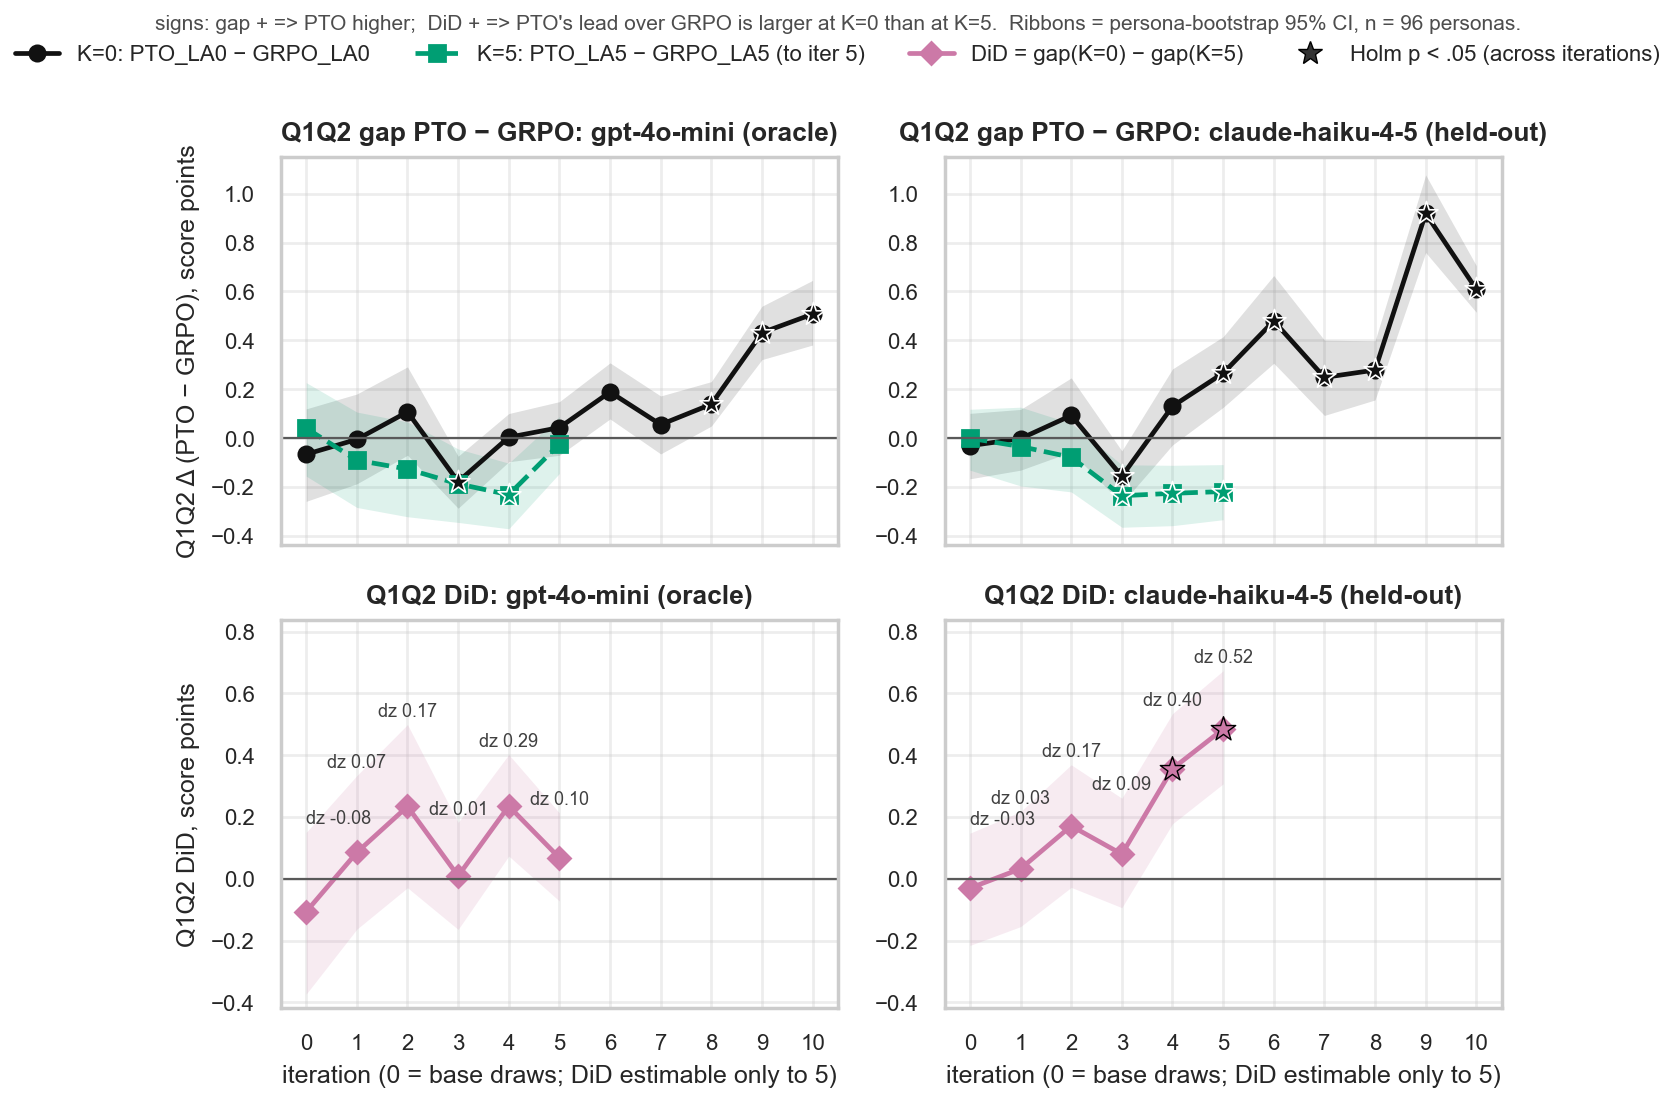
\includegraphics[width=\linewidth]{figures/cross_k_multijudge_fig_did.png}
  \caption{The method gap on \QQ{} at \Kz{} (solid, to iteration~10) and \Kf{} (dashed, to
    iteration~5) with 95\% CIs (top), and their persona-level difference (bottom), under each
    grader. Positive DiD: PTO's lead is larger at \Kz{}. Stars: Holm across iterations.}
  \label{fig:did}
\end{figure}

\begin{table}[t]
  \centering\scriptsize
  \setlength{\tabcolsep}{2pt}
  \begin{tabular}{@{}l c l ll c@{}}
    \toprule
    method & iter. & instr. & \Kz{} retention & \Kf{} retention & disjoint \\
    \midrule
PTO & 5 & Q1Q2 & $0.909$ $[0.79, 1.05]$ & $0.735$ $[0.63, 0.86]$ & no \\
PTO & 5 & Q1 & $0.975$ $[0.83, 1.15]$ & $0.827$ $[0.69, 0.98]$ & no \\
PTO & 5 & Q2 & $0.846$ $[0.73, 0.99]$ & $0.640$ $[0.53, 0.77]$ & no \\
PTO & 5 & MITI & $0.654$ $[0.54, 0.80]$ & $0.413$ $[0.29, 0.54]$ & no \\
PTO & 5 & MICI & $1.832$ $[0.94, 2.96]$ & $1.701$ $[1.21, 2.43]$ & no \\
\addlinespace[2pt]
PTO & 10 & Q1Q2 & $0.823$ $[0.72, 0.95]$ & $0.639$ $[0.55, 0.74]$ & no \\
PTO & 10 & Q1 & $0.795$ $[0.69, 0.93]$ & $0.720$ $[0.61, 0.84]$ & no \\
PTO & 10 & Q2 & $0.849$ $[0.75, 0.98]$ & $0.562$ $[0.48, 0.65]$ & yes \\
PTO & 10 & MITI & $0.450$ $[0.36, 0.55]$ & $0.268$ $[0.18, 0.35]$ & yes \\
PTO & 10 & MICI & $1.657$ $[1.30, 2.15]$ & $2.442$ $[1.50, 3.84]$ & no \\
\addlinespace[2pt]
GRPO & 5 & Q1Q2 & $0.691$ $[0.54, 0.86]$ & $0.893$ $[0.78, 1.02]$ & no \\
GRPO & 5 & Q1 & $0.786$ $[0.59, 1.00]$ & $1.048$ $[0.91, 1.22]$ & no \\
GRPO & 5 & Q2 & $0.608$ $[0.48, 0.77]$ & $0.738$ $[0.65, 0.85]$ & no \\
GRPO & 5 & MITI & $0.276$ $[0.12, 0.42]$ & $0.398$ $[0.31, 0.48]$ & no \\
GRPO & 5 & MICI & $3.713$ $[2.18, 5.06]$ & $2.440$ $[1.76, 3.80]$ & no \\
    \bottomrule
  \end{tabular}
  \caption{Own-base gain retention: (held-out gain over the arm's own base) $/$ (oracle gain over
    the same base), with persona-bootstrap 95\% CIs; ``disjoint'' flags non-overlapping intervals
    between the two $K$ arms. Under the \Kf{} arm's base as a shared reference the GRPO Q1 intervals
    at iteration~5 separate ($1.05$ vs $0.71$ $[0.54, 0.88]$); under the \Kz{} arm's base they
    still overlap ($1.16$ $[0.99, 1.39]$ vs $0.79$ $[0.59, 1.00]$); the two GRPO base draws differ
    by $0.104$ on \QQ{} under the training oracle ($0.026$ under the held-out judge).
    Source: \texttt{cross\_k\_multijudge\_retention\_summary}.}
  \label{tab:app:retention}
\end{table}

\begin{table*}[t]
  \centering\footnotesize
  \setlength{\tabcolsep}{4pt}
  \begin{tabular}{@{}l l rrl rrl@{}}
    \toprule
    & & \multicolumn{3}{c}{training oracle} & \multicolumn{3}{c}{held-out judge} \\
    \cmidrule(lr){3-5}\cmidrule(lr){6-8}
    pair (A $-$ B) & instr. & $\Delta$ & \dz{} & $p_{\text{Holm}}$ & $\Delta$ & \dz{} & $p_{\text{Holm}}$ \\
    \midrule
PTO~\Kz{} I10 $-$ GRPO~\Kz{} I10 & Q1Q2 & $+0.507$ & $+0.73$ & $<$.001 & $+0.609$ & $+1.27$ & $<$.001 \\
 & Q1 & $+0.533$ & $+0.71$ & $<$.001 & $+0.773$ & $+1.21$ & $<$.001 \\
 & Q2 & $+0.481$ & $+0.70$ & $<$.001 & $+0.445$ & $+0.93$ & $<$.001 \\
 & MITI & $+0.352$ & $+0.46$ & $<$.001 & $+0.253$ & $+0.65$ & $<$.001 \\
 & PCT & $+0.056$ & $+0.29$ & .015 & $+0.021$ & $+0.12$ & .204 \\
 & MICI & $-0.346$ & $-0.99$ & $<$.001 & $-0.224$ & $-0.67$ & $<$.001 \\
\addlinespace[2pt]
PTO~\Kf{} I10 $-$ GRPO~\Kf{} I5 & Q1Q2 & $+0.265$ & $+0.38$ & $<$.001 & $-0.131$ & $-0.19$ & .818 \\
 & Q1 & $+0.238$ & $+0.29$ & .015 & $-0.206$ & $-0.23$ & .384 \\
 & Q2 & $+0.293$ & $+0.47$ & $<$.001 & $-0.055$ & $-0.09$ & .818 \\
 & MITI & $+0.247$ & $+0.38$ & $<$.001 & $-0.036$ & $-0.09$ & .818 \\
 & PCT & $+0.060$ & $+0.27$ & .004 & $+0.062$ & $+0.26$ & .015 \\
 & MICI & $-0.077$ & $-0.29$ & .015 & $-0.066$ & $-0.17$ & .672 \\
\addlinespace[2pt]
PTO~\Kf{} I10 $-$ PTO~\Kz{} I10 & Q1Q2 & $+0.047$ & $+0.10$ & .695 & $-0.199$ & $-0.31$ & .129 \\
 & Q1 & $+0.085$ & $+0.14$ & .695 & $-0.035$ & $-0.04$ & 1.000 \\
 & Q2 & $+0.009$ & $+0.02$ & 1.000 & $-0.363$ & $-0.65$ & $<$.001 \\
 & MITI & $-0.016$ & $-0.03$ & 1.000 & $-0.203$ & $-0.49$ & $<$.001 \\
 & PCT & $+0.008$ & $+0.04$ & 1.000 & $+0.051$ & $+0.25$ & .017 \\
 & MICI & $-0.228$ & $-0.71$ & $<$.001 & $-0.245$ & $-0.66$ & $<$.001 \\
\addlinespace[2pt]
GRPO~\Kf{} I5 $-$ GRPO~\Kz{} I5 & Q1Q2 & $+0.070$ & $+0.13$ & .365 & $+0.311$ & $+0.43$ & .006 \\
 & Q1 & $+0.119$ & $+0.21$ & .205 & $+0.450$ & $+0.50$ & $<$.001 \\
 & Q2 & $+0.021$ & $+0.04$ & .365 & $+0.172$ & $+0.26$ & .183 \\
 & MITI & $+0.070$ & $+0.15$ & .365 & $+0.099$ & $+0.21$ & .171 \\
 & PCT & $+0.056$ & $+0.31$ & .022 & $+0.067$ & $+0.37$ & .004 \\
 & MICI & $+0.063$ & $+0.24$ & .205 & $+0.018$ & $+0.05$ & .636 \\
\addlinespace[2pt]
GRPO~\Kf{} I5 $-$ GRPO~\Kz{} I10 & Q1Q2 & $+0.289$ & $+0.36$ & .019 & $+0.541$ & $+0.84$ & $<$.001 \\
 & Q1 & $+0.381$ & $+0.42$ & $<$.001 & $+0.944$ & $+1.10$ & $<$.001 \\
 & Q2 & $+0.197$ & $+0.26$ & .553 & $+0.137$ & $+0.24$ & .087 \\
 & MITI & $+0.089$ & $+0.11$ & 1.000 & $+0.086$ & $+0.20$ & .130 \\
 & PCT & $+0.004$ & $+0.02$ & 1.000 & $+0.010$ & $+0.05$ & .806 \\
 & MICI & $-0.497$ & $-1.34$ & $<$.001 & $-0.403$ & $-1.23$ & $<$.001 \\
\addlinespace[2pt]
GRPO~\Kf{} I5 $-$ GRPO~\Kz{} I8 (oracle-best \Kz{}) & Q1Q2 & $-0.041$ & $-0.07$ & 1.000 & $+0.181$ & $+0.29$ & .089 \\
 & Q1 & $+0.052$ & $+0.07$ & 1.000 & $+0.485$ & $+0.60$ & $<$.001 \\
 & Q2 & $-0.134$ & $-0.22$ & .013 & $-0.124$ & $-0.22$ & .074 \\
 & MITI & $-0.224$ & $-0.40$ & $<$.001 & $-0.034$ & $-0.09$ & .853 \\
 & PCT & $+0.007$ & $+0.03$ & 1.000 & $+0.026$ & $+0.12$ & .853 \\
 & MICI & $-0.195$ & $-0.62$ & $<$.001 & $-0.252$ & $-0.62$ & $<$.001 \\
\addlinespace[2pt]
GRPO~\Kf{} I5 $-$ GRPO~\Kz{} I3 (judge-best \Kz{}) & Q1Q2 & $+0.048$ & $+0.10$ & .251 & $+0.161$ & $+0.31$ & .040 \\
 & Q1 & $+0.052$ & $+0.10$ & .290 & $+0.233$ & $+0.34$ & .020 \\
 & Q2 & $+0.044$ & $+0.10$ & .290 & $+0.089$ & $+0.17$ & .742 \\
 & MITI & $+0.073$ & $+0.15$ & .290 & $-0.198$ & $-0.44$ & $<$.001 \\
 & PCT & $+0.035$ & $+0.20$ & .105 & $+0.022$ & $+0.13$ & .742 \\
 & MICI & $+0.110$ & $+0.40$ & .002 & $+0.239$ & $+0.76$ & $<$.001 \\
    \bottomrule
  \end{tabular}
  \caption{Endpoint contrasts, A minus B as named (positive: A higher; on MICI, lower is better,
    so a negative value favours A). Holm across the nine instruments within a pair (WAI-SR, CSQ-8
    and MI-SAT rows omitted here). GRPO \Kz{}'s best iteration is grader-dependent (8 under the
    oracle, 3 under the judge); both are tabulated. Source: \texttt{cross\_k\_multijudge\_endpoints}.}
  \label{tab:app:endpoints}
\end{table*}

\begin{figure*}[t]
  \centering
  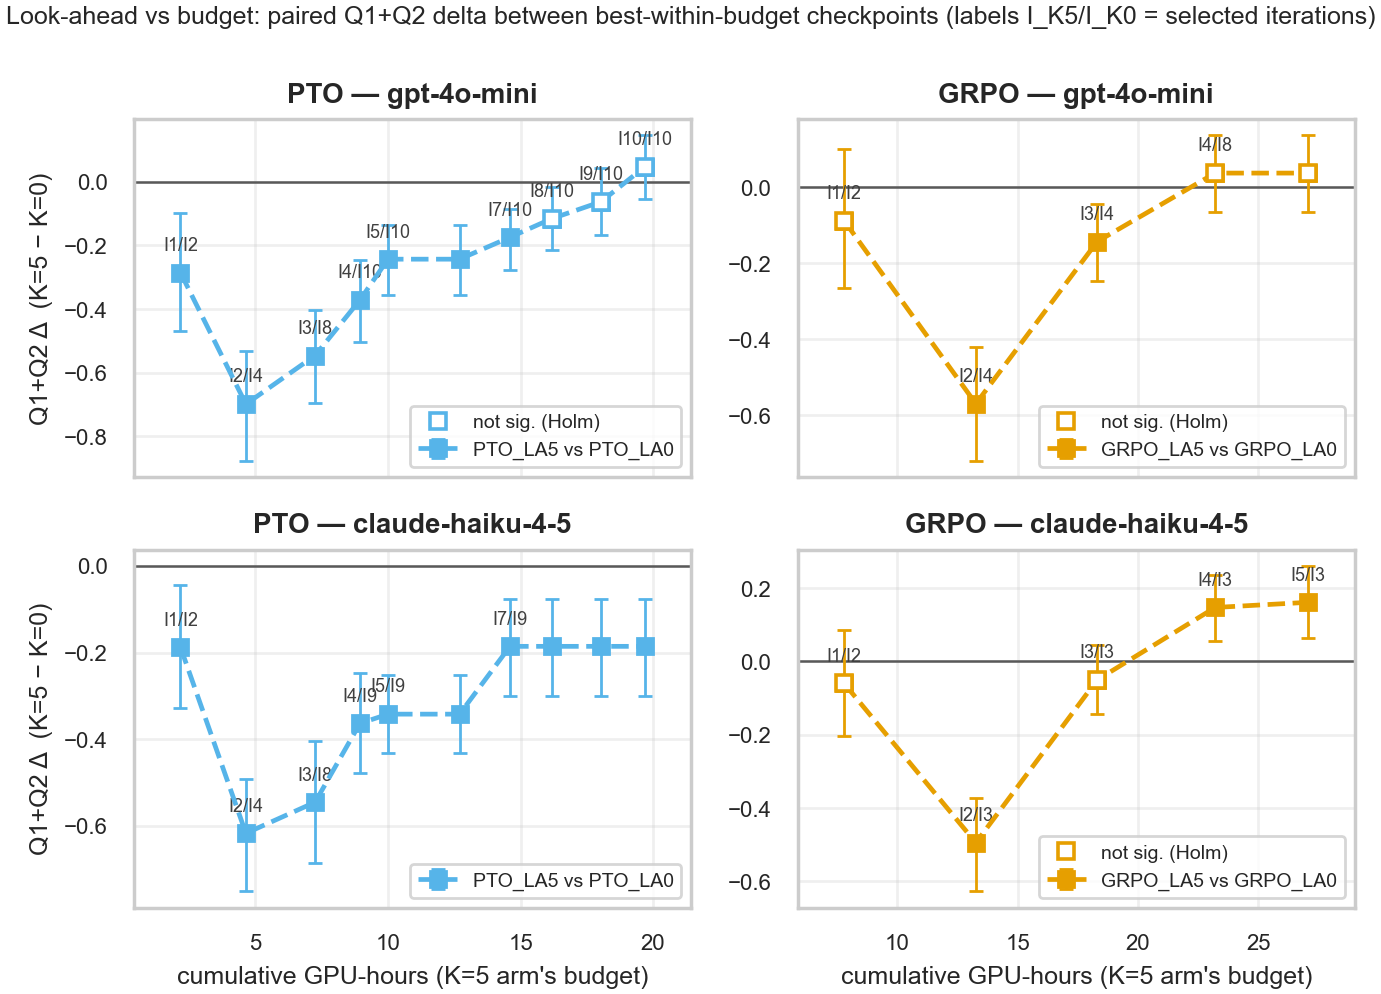
\includegraphics[width=\textwidth]{figures/compute_axis_fig_budget_sweep.png}
  \caption{Budget sweeps of the $K$ lever. Rows: grader; columns: method. At each of the \Kf{}
    arm's cumulative GPU-h budgets, the paired \QQ{} difference between the best-within-budget
    checkpoints of the two arms (selected on that grader's \QQ{}), $K{=}5$ minus $K{=}0$, with 95\%
    bootstrap CI; hollow markers do not clear Holm; labels give the selected iterations. GRPO
    \Kf{} ends at $27.1$\,\gpuh{}.}
  \label{fig:sweep}
\end{figure*}

\begin{table*}[t]
  \centering\footnotesize
  \setlength{\tabcolsep}{4pt}
  \begin{tabular}{@{}l r c rrlr@{}}
    \toprule
    contrast, grader & budget (\gpuh{}) & iters (\Kf{}/\Kz{}) & $\Delta$ (\Kf{}$-$\Kz{}) & \dz{} & 95\% CI & $p_{\text{Holm}}$ \\
    \midrule
PTO $K$, oracle & $2.17$ & 1/2 & $-0.286$ & $-0.30$ & $[-0.485, -0.087]$ & .046 \\
PTO $K$, oracle & $4.64$ & 2/4 & $-0.700$ & $-0.81$ & $[-0.871, -0.528]$ & $<$.001 \\
PTO $K$, oracle & $7.25$ & 3/8 & $-0.546$ & $-0.73$ & $[-0.703, -0.405]$ & $<$.001 \\
PTO $K$, oracle & $8.94$ & 4/10 & $-0.372$ & $-0.56$ & $[-0.505, -0.246]$ & $<$.001 \\
PTO $K$, oracle & $10.00$--$12.70$ & 5/10 & $-0.243$ & $-0.43$ & $[-0.356, -0.135]$ & $<$.001 \\
PTO $K$, oracle & $14.60$ & 7/10 & $-0.174$ & $-0.35$ & $[-0.277, -0.079]$ & .012 \\
PTO $K$, oracle & $16.17$ & 8/10 & $-0.116$ & $-0.23$ & $[-0.227, -0.017]$ & .190 \\
PTO $K$, oracle & $18.03$ & 9/10 & $-0.063$ & $-0.11$ & $[-0.176, +0.046]$ & .867 \\
PTO $K$, oracle & $19.68$ & 10/10 & $+0.047$ & $+0.10$ & $[-0.054, +0.142]$ & .190 \\
\addlinespace[2pt]
PTO $K$, held-out & $2.17$ & 1/2 & $-0.188$ & $-0.26$ & $[-0.330, -0.046]$ & .015 \\
PTO $K$, held-out & $4.64$ & 2/4 & $-0.617$ & $-0.94$ & $[-0.749, -0.492]$ & $<$.001 \\
PTO $K$, held-out & $7.25$ & 3/8 & $-0.546$ & $-0.76$ & $[-0.691, -0.405]$ & $<$.001 \\
PTO $K$, held-out & $8.94$ & 4/9 & $-0.364$ & $-0.61$ & $[-0.482, -0.252]$ & $<$.001 \\
PTO $K$, held-out & $10.00$--$12.70$ & 5/9 & $-0.342$ & $-0.74$ & $[-0.438, -0.248]$ & $<$.001 \\
PTO $K$, held-out & $14.60$--$19.68$ & 7/9 & $-0.186$ & $-0.32$ & $[-0.301, -0.072]$ & .011 \\
\addlinespace[2pt]
GRPO $K$, oracle & $7.80$ & 1/2 & $-0.088$ & $-0.09$ & $[-0.274, +0.099]$ & .814 \\
GRPO $K$, oracle & $13.27$ & 2/4 & $-0.569$ & $-0.74$ & $[-0.727, -0.422]$ & $<$.001 \\
GRPO $K$, oracle & $18.31$ & 3/4 & $-0.143$ & $-0.28$ & $[-0.247, -0.044]$ & .040 \\
GRPO $K$, oracle & $23.21$--$27.08$ & 4/8 & $+0.038$ & $+0.07$ & $[-0.053, +0.137]$ & .814 \\
\addlinespace[2pt]
GRPO $K$, held-out & $7.80$ & 1/2 & $-0.060$ & $-0.08$ & $[-0.204, +0.091]$ & .690 \\
GRPO $K$, held-out & $13.27$ & 2/3 & $-0.495$ & $-0.78$ & $[-0.620, -0.367]$ & $<$.001 \\
GRPO $K$, held-out & $18.31$ & 3/3 & $-0.051$ & $-0.11$ & $[-0.144, +0.043]$ & .690 \\
GRPO $K$, held-out & $23.21$ & 4/3 & $+0.147$ & $+0.33$ & $[+0.060, +0.236]$ & .012 \\
GRPO $K$, held-out & $27.08$ & 5/3 & $+0.161$ & $+0.31$ & $[+0.057, +0.263]$ & .020 \\
    \bottomrule
  \end{tabular}
  \caption{Budget sweep of the $K$ lever, both methods, both graders (Figure~\ref{fig:sweep}).
    Best-within-budget checkpoints selected on the same grader's \QQ{}; sign here is $K{=}5$ minus
    $K{=}0$; Holm within (grader, contrast) over unique checkpoint pairs. Budgets at which neither
    arm reaches a new checkpoint repeat the previous pair and are collapsed into a range. Source:
    \texttt{compute\_axis\_budget\_sweep\_PTO\_K\_*}, \texttt{\ldots\_GRPO\_K\_*}.}
  \label{tab:app:sweepK}
\end{table*}

\begin{table*}[t]
  \centering\footnotesize
  \setlength{\tabcolsep}{4pt}
  \begin{tabular}{@{}l r c rrlr@{}}
    \toprule
    $K$, grader & budget (\gpuh{}) & iters (PTO/GRPO) & $\Delta$ (PTO$-$GRPO) & \dz{} & 95\% CI & $p_{\text{Holm}}$ \\
    \midrule
\Kz{}, oracle & $2.80$ & 3/1 & $+0.546$ & $+0.54$ & $[+0.353, +0.759]$ & $<$.001 \\
\Kz{}, oracle & $3.90$ & 4/1 & $+0.739$ & $+0.81$ & $[+0.561, +0.925]$ & $<$.001 \\
\Kz{}, oracle & $4.66$ & 5/1 & $+0.745$ & $+0.78$ & $[+0.562, +0.944]$ & $<$.001 \\
\Kz{}, oracle & $5.37$--$6.07$ & 6/2 & $+0.795$ & $+0.91$ & $[+0.621, +0.972]$ & $<$.001 \\
\Kz{}, oracle & $6.88$ & 8/2 & $+0.861$ & $+0.99$ & $[+0.689, +1.044]$ & $<$.001 \\
\Kz{}, oracle & $7.49$ & 9/2 & $+0.879$ & $+1.07$ & $[+0.718, +1.050]$ & $<$.001 \\
\Kz{}, oracle & $8.12$ & 10/2 & $+0.900$ & $+1.09$ & $[+0.744, +1.074]$ & $<$.001 \\
\addlinespace[2pt]
\Kz{}, held-out & $2.80$ & 3/1 & $+0.406$ & $+0.58$ & $[+0.269, +0.542]$ & $<$.001 \\
\Kz{}, held-out & $3.90$ & 4/1 & $+0.606$ & $+0.84$ & $[+0.464, +0.743]$ & $<$.001 \\
\Kz{}, held-out & $4.66$ & 5/1 & $+0.678$ & $+0.96$ & $[+0.540, +0.823]$ & $<$.001 \\
\Kz{}, held-out & $5.37$--$6.07$ & 6/2 & $+0.743$ & $+1.14$ & $[+0.617, +0.873]$ & $<$.001 \\
\Kz{}, held-out & $6.88$ & 8/2 & $+0.789$ & $+1.34$ & $[+0.671, +0.907]$ & $<$.001 \\
\Kz{}, held-out & $7.49$--$8.12$ & 9/2 & $+0.814$ & $+1.39$ & $[+0.697, +0.929]$ & $<$.001 \\
\addlinespace[2pt]
\Kf{}, oracle & $8.94$ & 4/1 & $+0.616$ & $+0.64$ & $[+0.432, +0.815]$ & $<$.001 \\
\Kf{}, oracle & $10.00$--$12.70$ & 5/1 & $+0.745$ & $+0.81$ & $[+0.564, +0.941]$ & $<$.001 \\
\Kf{}, oracle & $14.60$ & 7/2 & $+0.650$ & $+0.78$ & $[+0.485, +0.820]$ & $<$.001 \\
\Kf{}, oracle & $16.17$ & 8/2 & $+0.709$ & $+0.89$ & $[+0.554, +0.880]$ & $<$.001 \\
\Kf{}, oracle & $18.03$ & 9/2 & $+0.762$ & $+0.92$ & $[+0.603, +0.941]$ & $<$.001 \\
\Kf{}, oracle & $19.68$ & 10/3 & $+0.445$ & $+0.67$ & $[+0.313, +0.583]$ & $<$.001 \\
\addlinespace[2pt]
\Kf{}, held-out & $8.94$ & 4/1 & $+0.511$ & $+0.71$ & $[+0.366, +0.653]$ & $<$.001 \\
\Kf{}, held-out & $10.00$--$12.70$ & 5/1 & $+0.533$ & $+0.79$ & $[+0.396, +0.663]$ & $<$.001 \\
\Kf{}, held-out & $14.60$--$18.03$ & 7/2 & $+0.594$ & $+0.82$ & $[+0.454, +0.737]$ & $<$.001 \\
\Kf{}, held-out & $19.68$ & 7/3 & $+0.149$ & $+0.29$ & $[+0.051, +0.248]$ & .007 \\
    \bottomrule
  \end{tabular}
  \caption{Budget sweep of the optimizer contrast at each $K$ (PTO minus GRPO; positive: PTO
    higher), on the PTO arm's cumulative budgets. Same selection and Holm conventions as
    Table~\ref{tab:app:sweepK}. At \Kf{} the sweep stops at PTO \Kf{}'s $19.68$\,\gpuh{}, where GRPO
    \Kf{} has reached iteration~3 of its five. Source:
    \texttt{compute\_axis\_budget\_sweep\_method\_K0\_*}, \texttt{\ldots\_K5\_*}.}
  \label{tab:app:sweepMethod}
\end{table*}

\paragraph{Cross-judge sweep verdicts.} Selecting the best-within-budget checkpoint on one grader
and scoring it on the other, at the top budget of each contrast (\QQ{}, persona-paired, Holm as
in Table~\ref{tab:app:sweepK}). GRPO $K$ ($K{=}5$ minus $K{=}0$): oracle selects, judge scores
$+0.166$ (\dz{} $0.27$, CI $[0.041, 0.291]$, $p_{\text{Holm}}{=}.035$; iteration~4 vs~8); judge
selects, oracle scores $+0.048$ (\dz{} $0.10$, n.s.). PTO $K$: judge selects, oracle scores
$-0.153$ (\dz{} $-0.27$, $p_{\text{Holm}}{=}.023$); oracle selects, judge scores $-0.199$
(\dz{} $-0.31$, $p_{\text{Holm}}{=}.065$). Method at \Kf{} (PTO minus GRPO), oracle selects,
judge scores: $+0.081$ (\dz{} $0.13$, CI $[-0.040, 0.199]$, $p_{\text{Holm}}{=}.075$). Source:
\texttt{compute\_axis\_budget\_sweep\_}\allowbreak\texttt{crossjudge\_verdicts}.
